
\documentclass[12pt]{article}

% Layout.
\usepackage[top=1in, bottom=0.75in, left=1in, right=1in, headheight=1in, headsep=6pt]{geometry}

% Fonts.
\usepackage{mathptmx}
\usepackage[scaled=0.86]{helvet}
\renewcommand{\emph}[1]{\textsf{\textbf{#1}}}

% TiKZ.
\usepackage{tikz, pgfplots}
\usetikzlibrary{calc}
\pgfplotsset{compat = newest}
 
\pgfplotsset{my style/.append style={axis x line=middle, axis y line=
middle, xlabel={$x$}, ylabel={$y$}, axis equal }}

% Misc packages.
\usepackage{amsmath,amssymb,latexsym}
\usepackage{graphicx}
\usepackage{array}
\usepackage{xcolor}
\usepackage{multicol}

% Commands to set various header/footer components.
\makeatletter
\def\doctitle#1{\gdef\@doctitle{#1}}
\doctitle{Use {\tt\textbackslash doctitle\{MY LABEL\}}.}
\def\docdate#1{\gdef\@docdate{#1}}
\docdate{Use {\tt\textbackslash docdate\{MY DATE\}}.}
\def\doccourse#1{\gdef\@doccourse{#1}}
\let\@doccourse\@empty
\def\docscoring#1{\gdef\@docscoring{#1}}
\let\@docscoring\@empty
\def\docversion#1{\gdef\@docversion{#1}}
\let\@docversion\@empty
\makeatother

% Headers and footers layout.
\makeatletter
\usepackage{fancyhdr}
\pagestyle{fancy}
\fancyhf{} % Clears all headers/footers.
\lhead{\baselineskip 30pt
%\emph{\@doctitle\hfill\@docdate}
\emph{\@docdate\hfill\@doctitle}
\ifnum \value{page} > 1\relax\else\\
\emph{Name: \rule{3.5in}{1pt}\hfill \@docscoring}\fi}
\rfoot{\emph{\@docversion}}
\lfoot{\emph{\@doccourse}}
\cfoot{\emph{\thepage}}
\renewcommand{\headrulewidth}{0pt}%
\makeatother

% Paragraph spacing
\parindent 0pt
\parskip 6pt plus 1pt

% A problem is a section-like command. Use \problem{5} to
% start a problem worth 5 points.
\newcounter{probcount}
\newcounter{subprobcount}
\setcounter{probcount}{0}
\newcommand{\problem}[1]{%
\par
\addvspace{4pt}%
\setcounter{subprobcount}{0}%
\stepcounter{probcount}%
\makebox[0pt][r]{\emph{\arabic{probcount}.}\hskip1ex}\emph{[#1 points]}\hskip1ex}
\newcommand{\thesubproblem}{\emph{\alph{subprobcount}.}}

% Subproblems are an enumerate-like environment with a consistent
% numbering scheme. 
% Use \begin{subproblems}\item...\item...\end{subproblems}
\newenvironment{subproblems}{%
\begin{enumerate}%
\setcounter{enumi}{\value{subprobcount}}%
\renewcommand{\theenumi}{\emph{\alph{enumi}}}}%
{\setcounter{subprobcount}{\value{enumi}}\end{enumerate}}

% Blanks for answers in normal and math mode.
\newcommand{\blank}[1]{\rule{#1}{0.75pt}}
\newcommand{\mblank}[1]{\underline{\hspace{#1}}}
\def\emptybox(#1,#2){\framebox{\parbox[c][#2]{#1}{\rule{0pt}{0pt}}}}

% Misc.
\renewcommand{\d}{\displaystyle}
\newcommand{\ds}{\displaystyle}
\def\bc{\begin{center}}
\def\ec{\end{center}}
\def\be{\begin{enumerate}}
\def\ee{\end{enumerate}}


\doctitle{Math 251: Quiz 3}
\docdate{Sept 15, 2022}
\doccourse{UAF Calculus I}
\docversion{v-1}
\docscoring{\blank{0.8in} / 25}
\begin{document}
%\textbf{Please circle your instructor's name:} \hfill Leah Berman  \hfill   Jill Faudree\\

There are 25 points possible on this quiz. No aids (book, calculator, etc.)
are permitted.  {\bf Show all work for full credit.}

\begin{enumerate}
\item (10 points) Use the graph of the function $H(x)$ (drawn below) to answer the questions. Assume $H(x)$ has a vertical asymptote at $x=5.$ For each problem below, give the most complete answer; if the limit is infinite, indicate that with $\infty$ or $-\infty.$ \\

\begin{center}
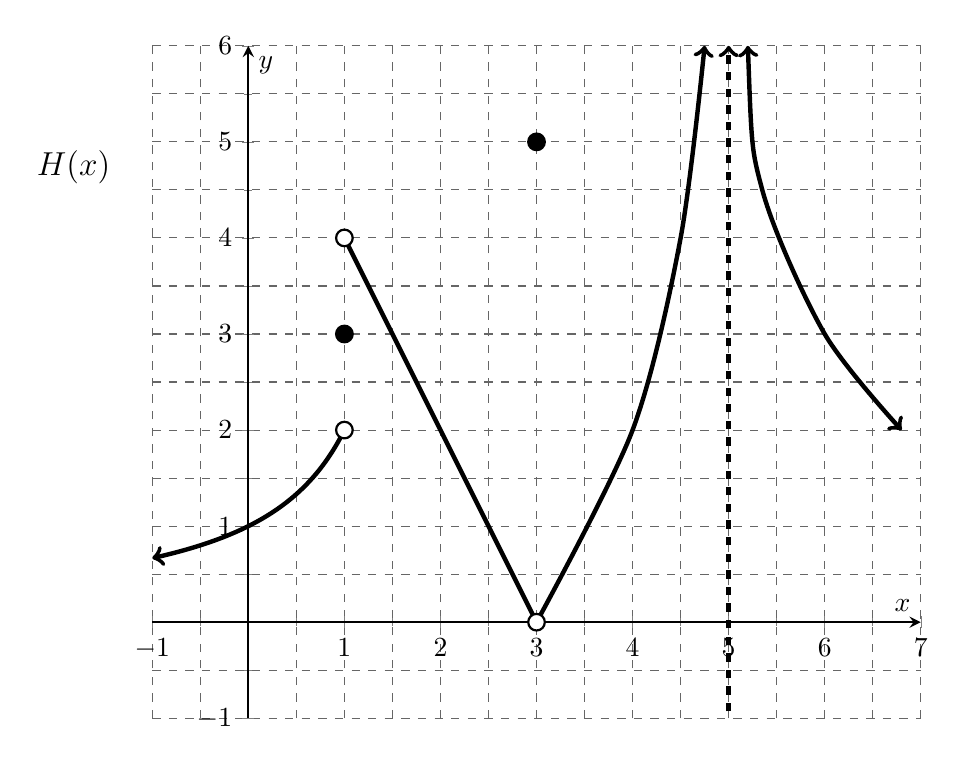
\begin{tikzpicture}
\begin{axis}[scale=1.5, thick, my style, xtick={-2,...,7}, ytick={-1, 0,...,6},
xmin=-1, xmax=7, ymin=-1, ymax=6, minor y tick num=1,
        minor x tick num=1, mark size=3.0pt, grid=both, grid style={ thin, black!60, dashed}, axis equal image]
% %%asymptote
\addplot[dashed,<->, ultra thick] coordinates {(5,-2) (5,6)};       
%%points solid
\addplot[mark=*,only marks] coordinates {(1,3)(3,5)};
%%points open
\addplot[mark=*,fill=white,only marks] coordinates {(1,2)(1,4)(3,0)};
%%Curves
\addplot[<-,ultra thick, smooth, variable=\x, samples=100, domain=-1:1] plot(\x,{-2/(\x-2)});
%\addplot[ultra thick, smooth,<-] coordinates {(-3,4) (-2,3.5) (0,2)(1,0.5)};
\addplot[ultra thick, smooth] coordinates {(1,4) (3,0)};
\addplot[ultra thick, smooth,->] coordinates {(3,0) (4,2) (4.5,4)(4.75,6)};
%\addplot[ultra thick, smooth,->] coordinates {(2,2) (2.5,2.3) (2.7,4.5) (2.8,6)};
\addplot[ultra thick, smooth,<->] coordinates {(5.2,6) (5.35,4.5) (6,3)(6.8,2)};       
\end{axis}
\node at (-1,7){\large{$H(x)$}};
\end{tikzpicture}
\end{center}

\begin{enumerate}
\begin{multicols}{3}
\item $H(0)=\mblank{.5in}$
\item $H(1)=\mblank{.5in}$
\item $H(3)=\mblank{.5in}$
%\item $f(5)=\mblank{.5in}$
\end{multicols}
\vspace{0.1in}
\begin{multicols}{3}
\item $\d{\lim_{x \to\; 1^-} H(x)=\mblank{.5in}}$
\item $\d{\lim_{x \to\; 1^+} H(x)=\mblank{.5in}}$
\item $\d{\lim_{x \to\; 1} H(x)=\mblank{.5in}}$
\end{multicols}
\vspace{0.1in}
\begin{multicols}{3}
\item $\d{\lim_{x \to 0} H(x)=\mblank{.5in}}$
\item $\d \lim_{x\to\; 3}H(x)=\mblank{.5in}$
\item $\d{\lim_{x \to 5} H(x)=\mblank{.5in}}$
\end{multicols}
\vspace{0.1in}
\item List all $x$-values for which the function $H(x)$ fails to be continuous.\\
\vfill

\end{enumerate}
\newpage
\item (12 points) Evaluate the following limits. Show your work to earn full credit.
	\begin{enumerate}
	\item $\displaystyle{\lim_{x  \to -1}\frac{x^2-1}{x+1}}=$
	\vfill
	\item $\displaystyle{\lim_{x  \to 0}\frac{\frac{2}{3+x}-\frac{2}{3}}{x}}=$
	\vfill
	\item $\displaystyle{\lim_{x  \to 5^+}\frac{1+\sqrt{x+4}}{5-x}}=$
	\vfill
	\item If  $\displaystyle{\lim_{x  \to 2}f(x)=7}$, find $\displaystyle{\lim_{x  \to 2}(5-2x+3f(x))}=$
	\vfill
	\end{enumerate}
\item (3 points) Pick $k$ such that $f(x)$ is continuous if $f(x)=\begin{cases} x^2 & x\leq 2 \\ 3x+k&x>2 \end{cases}.$
\vfill
\end{enumerate}	
\end{document}